\chapter{Additional Pipeline Information}
\section{Corner thresholding}
\label{sec:corner_thresholding}
describe the corner thresholding approach here.

\section{Depth Field Variances}
\label{sec:depth_field_variances}
describe how depth field variances can be computed and how they can be used. Additionally, describe the run-mode in the pipeline and maybe also offer some results and limitations.

\chapter{Additional Theoretical Background}
\section{On Filtering Images}
\subsection{Gaussian Filter}
A Gaussian filter (\textbf{GF}) is a linear operator that reduces noise by smoothing the image. Applying GF corresponds to a low-pass filtering.
At each position it estimates a local average of the intensities as defined in equation $\ref{eq:gaussian_filtering_def}$.
\begin{equation}
	\mathcal{F}^{\text{gf}} \{I \} (p) = \sum_{q \in \Omega_p} G_{\sigma} (\norm{p - q}) I_q
\label{eq:gaussian_filtering_def}
\end{equation}
where $I$ defines the input image and $\Omega_p$ contains all neighboring points within the window that are centered at the image point $p$. Moreover, $G_{\sigma}$ denotes the two dimensional Gaussian kernel, which is defined in equation $\ref{eq:def_g_weight}$.
\begin{equation}
	G_{\sigma} (x) = \frac{1}{2 \pi \sigma^2} e^{-\frac{x^2}{2 \sigma^2}}
\label{eq:def_g_weight}
\end{equation}
The Gaussian filtering is the weighted average of the intensity of the adjacent positions with a weight decreasing with the spatial distance to the center position. This distance is defined by $G_{\sigma} (\norm{p - q})$ where $\sigma$ is a parameter that defines the size of the neighborhood. The resulting image is a blurred version of the input image.

\subsection{Bilateral Filter}
A Bilateral filter (\textbf{BF}) is a non-linear operator that reduces noise by smoothing the image but at the same time preserves its edges. \\ \\
The rational of this filter is that two pixels are close to each other if not only if their spacial distance is small but also if they are similar regarding their intensity range.
\begin{figure}[H]
\begin{center}
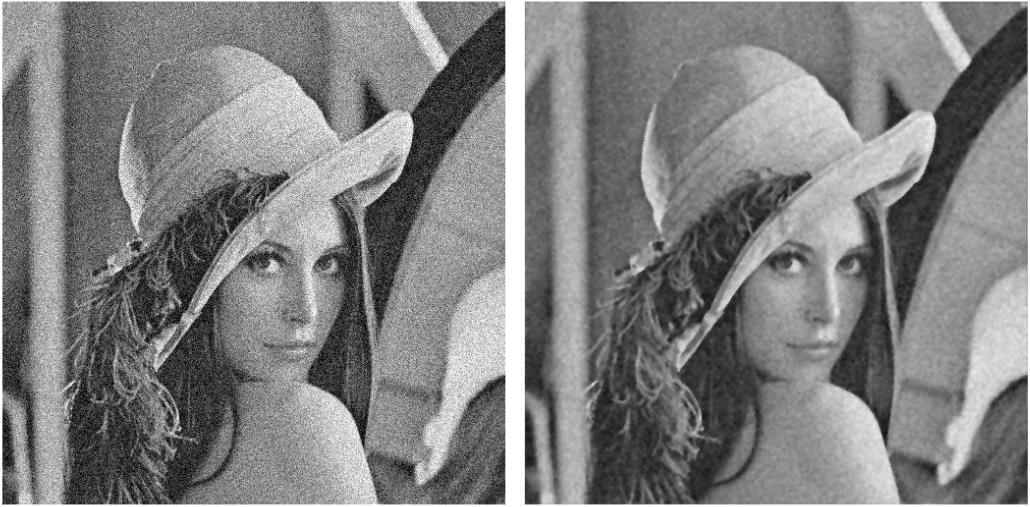
\includegraphics[width=0.6\linewidth] {background/filtering/bilat_filter_eg}
\end{center}
\caption[Example Bilateral Filter]{A bilateral filtering example$\footnotemark$: On the left side a noisy input image on the right its bilateral filtered version.}
\label{fig:bilat_filtering_eg}
\end{figure}
\footnotetext{The shown images have been extracted from: \\ \url{https://www.uni-due.de/mathematik/krommweh/talk_Gemen_Krommweh.pdf}}
The filter replaces the intensity values at each pixel in an image by a weighted average of intensity values from nearby pixels. In our formulation we rely on the Gaussian distributions $G$ for defining the weights. Crucially, the weights depend not only on distances between pixels, but also on the intensity difference. That is why, when iterating through each pixel and adjusting weights to the adjacent pixels accordingly, Sharp edges are preserved. A bilateral filtering example is shown in figure $\ref{fig:bilat_filtering_eg}$.\\ \\
The mathematical definition of this filter is given in equation $\ref{eq:def_bilateral_filter}$. For a given Image $I$ we want to compute its bilateral filtered version by applying the following definition:
\begin{equation}
\begin{aligned}
&\mathcal{F}^{\text{bf}} \{I \} (p) = \frac{1}{W_p} \sum_{q \in \Omega_p} G_{\sigma_s} (\norm{p-q})G_{\sigma_r} (I_p - I_q) I_q \\	
& \text{where } W_p = \sum_{q \in \Omega_p} G_{\sigma_s} (\norm{p-q})G_{\sigma_r} (I_p - I_q)
\end{aligned}
\label{eq:def_bilateral_filter}
\end{equation}
The set $\Omega_p$ contains all neighboring points within the window that are centered at the image point $p$. The scalar $W_p$ denotes the normalization factor of the filter and $I_p$ represents the image intensity at the pixel position $p$. Please notice that the definition of the bilateral filter is given per pixel, i.e. gives an representation of the filtered pixel intensity. \\ \\
The bilateral filter is controlled by the two parameters $\sigma_s$ and $\sigma_r$. The range variance increases $\sigma_r$, the BF becomes closer to the Gaussian blur filter. In other words, the larger $\sigma_r$ the more weight a pixel with a large intensity deviation gets. However, when increasing the spatial variance $\sigma_s$ results in smoothing larger features, i.e more distant pixels get a larger weight and thus influence the result more. Figure $\ref{fig:bfilter_influence_sigmas}$ demonstrates the influence of these parameters.
\begin{figure}[H]
\begin{center}
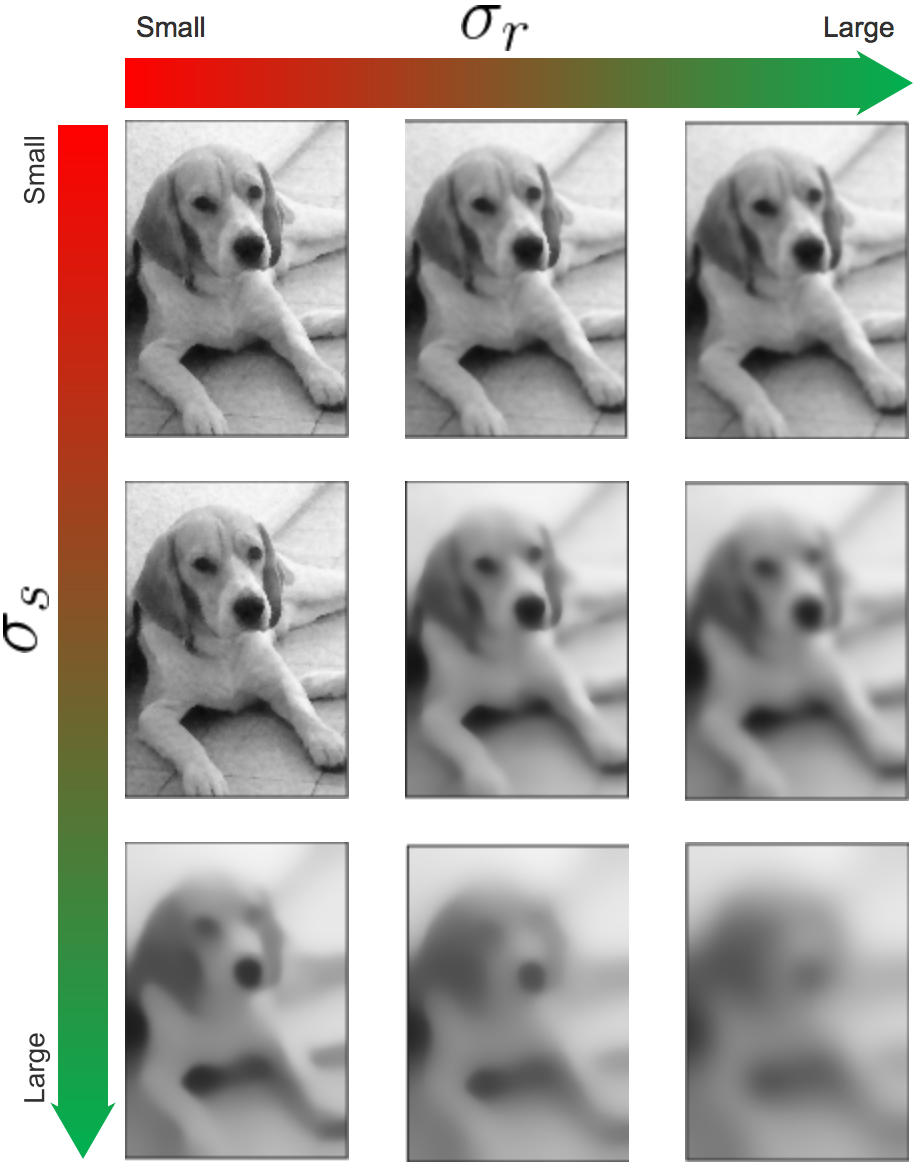
\includegraphics[width=0.6\linewidth] {background/filtering/bilat_filter_sigmas}
\end{center}
\caption[Influence of $\sigma_s$ and $\sigma_r$]{Different filtering results produced by our bilateral filter implementation for varying $\sigma_s$ and $\sigma_r$ values.}
\label{fig:bfilter_influence_sigmas}
\end{figure}

\subsection{Harris Corner Detector}
\label{sec:harris_corner_detector}
Let us consider a grayscale image $I$. We are going to sweep a window $w(x,y)$ (with displacements u in the x direction and v in the right direction) I and will calculate the variation of intensity. Since we are looking for windows with corners, we are looking for windows with a large variation in intensity. Hence, we have to maximize the equation above, specifically the term:
\begin{equation}
	E \left( u, v \right) = \sum_{x,y} w \left( x,y \right) \left[ I(x + u, y + v) - I(x, y) \right]^2
\label{eq:var_intensitiy_def}
\end{equation}
Next, the term $I(x + u, y + v)$ is expressed by the first order taylor series expansion as the follows:
\begin{equation}
	I(x + u, y + v) = I(x,y) + u I_x (x, y) + v I_y (x,y) + \text{h.o.t}
\label{eq:taylor_exp_intensity}
\end{equation}
Next, we put the first order approximation of equation $\ref{eq:taylor_exp_intensity}$ into equation $\ref{eq:var_intensitiy_def}$ to simplify the definition of $E$.
\begin{equation}
\begin{aligned}
E \left( u, v \right) 
&= \sum_{x,y} w \left( x,y \right) \left[ I(x + u, y + v) - I(x, y) \right]^2 \\
&\approx \sum_{x,y} w \left( x,y \right) \left[ I(x,y) + u I_x (x, y) + v I_y (x,y) - I(x, y) \right]^2 \\
&= \sum_{x,y} w \left( x,y \right) \left[ u I_x (x, y) + v I_y (x,y) \right]^2 \\
&= \sum_{x,y} w \left( x,y \right) u^2 I_x^2 + 2 u v I_x I_y v^2 I_y^2 \\
&= \left( u,v \right) \left( \sum_{x,y} w (x,y)
\begin{pmatrix}
I_x^2 & I_x I_y \\
I_x I_y & I_y^2 \\
\end{pmatrix}
\right) \colvec{u}{v}
\end{aligned}
\label{eq:var_intensitiy_developed}
\end{equation}
Let us define the following substitution
\begin{equation}
M = \sum_{x,y} w  (x,y)
\begin{pmatrix}
I_x^2 & I_x I_y \\
I_y^2 & I_x I_y \\
\end{pmatrix}
\label{eq:var_intensity_sub}
\end{equation}
Putting the substitution from equation $\ref{eq:var_intensity_sub}$ into the final form of equation $\ref{eq:var_intensitiy_developed}$ we obtain the final form
\begin{equation}
	E \left( u, v \right) \approx \left( u,v \right) M \colvec{u}{v}
\end{equation}.
A score is calculated for each window, to determine if it can possibly contain a corner:
\begin{equation}
\begin{aligned}
& R = \det(M) - \kappa \left(\text{trace}(M)\right)^2 \\
&\text{where } \det(M) = \lambda_1 \lambda_2 \text{ and } \text{trace}(M) = \lambda_1 + \lambda_2
\end{aligned}
\label{eq:harris_response}
\end{equation}

\section{On Statistics}
\label{sec:on_statistics_bg}

\subsection{Conditional Probability}
Given two events $A$ and $B$ with the probability $P(B) > 0$. The conidtional probability of $A$ given $B$ is defined as
\begin{equation}
	P(A|B) = \frac{P(A \cap B)}{P(B)}
\label{eq:conditional_prob}
\end{equation}
Furthermore, equation $\ref{eq:conditional_prob}$ gives us an alternative interpretation of the probability of an intersection
\begin{equation}
P(A \cap B) = P(A|B)P(B) 	
\end{equation}
The probability that two events happen the same time is the same as the Probability of the event A given B times the probability of event B. Sticking to this definition, we can visualize all possible outcomes of two events happening the same time as shown in figure $\ref{fig:prob_tree_diagram}$.
\begin{figure}[H]
\begin{center}
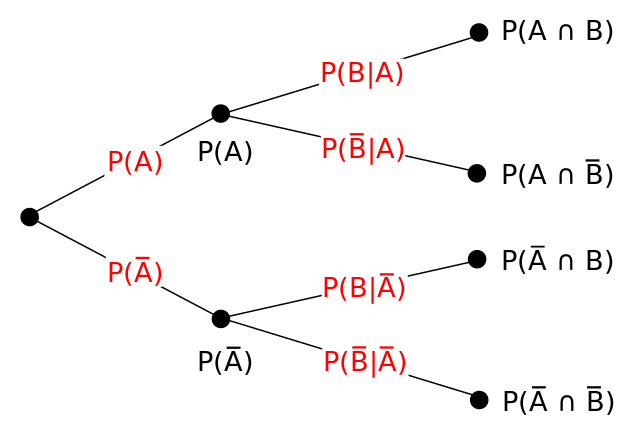
\includegraphics[width=0.45\linewidth] {background/statistics/probability_tree_diagram}
\end{center}
\caption[Probability Tree Diagram]{Tree liked representation$\footnotemark$ of the four possible outcomes for a conditional probability.}
\label{fig:prob_tree_diagram}
\end{figure}
\footnotetext{The visualized graphic has been taken from: \url{https://en.wikipedia.org/wiki/File:Probability_tree_diagram.svg}}



\subsection{Evaluating Binary Classifiers}
In this section we explain the mathematical framework we use in our evaluation.


The purpose of a binary classifier is to classify given elements into two groups according to a specified classification rule. Think about a binary random variable modelling a certain event. The actual observations of the random variable are then either equals true or false. A classification$\footnote{I.e. the produced output after applying the classifier on the given data.}$ of a given dataset yields two numbers: the number of the positives and negatives, which add up to the size of the set. \\ \\
In order to evaluate the quality of binary classifier its prediction is compared against a standard reference method or, if existing, against a ground truth assignment and then cross tabulates the data into a $2 \times 2$ contingency table as shown in figure $\ref{tab:prediction_sensitivity}$. 
\begin{table}[H]
\centering
\begin{tabular}{c|c|c|}
\cline{2-3}
 & \begin{tabular}[c]{@{}l@{}}Prediction\\ Positive\end{tabular} & \begin{tabular}[c]{@{}l@{}}Prediction\\ Negative\end{tabular} \\ \hline
\multicolumn{1}{|l|}{\begin{tabular}[c]{@{}l@{}}Condition\\ Positive\end{tabular}} & \cellcolor[HTML]{34FF34}{\color[HTML]{000000} $\bf{TP}$ } & \cellcolor[HTML]{CB0000} $\bf{FN}$ \\ \hline
\multicolumn{1}{|l|}{\begin{tabular}[c]{@{}l@{}}Condiation\\ Negative\end{tabular}} & \cellcolor[HTML]{CB0000}{\color[HTML]{000000} $\bf{FP}$ } & \cellcolor[HTML]{34FF34} $\bf{TN}$ \\ \hline
\end{tabular}
\caption[Conditional Probability]{The four possible outcomes of a conditional probability}
\label{tab:prediction_sensitivity}
\end{table}
There are four possible outcomes: the classifier prediction, which has either are positive or negative condition, was actually correct or incorrect. \\ \\
Let us consider the following example where we test some people for the presence of a disease. Some of these people have the disease, and the test correctly detects them. These findings are called true positives (\textbf{TP}). Some have the disease, but the test incorrectly claims that they do not have it. These results are called false negatives (\textbf{FN}). Some people do not suffer from the disease and the test classifies correctly as health. These results are called true negatives (\textbf{TN}). And Lastly, some healthy people who are incorrectly classified as infected. These are the so called false positives (\textbf{FP}) results. \\ \\
There are many metrics that can be used to measure the performance of a classifier. In the following a listing of some prominent metrics
%
\begin{itemize}
\item \textbf{Precision}: Tells us what proportion of patients we diagnosed as having the disease actually had that disease. In other words, proportion of TP in the set of positive disease diagnoses. This is given by the rightmost column in the confusion matrix.
\begin{equation}
	\text{precision} = \frac{\text{TP}}{\text{TP} + \text{FP}}
\label{eq:def_precision}
\end{equation}
\item \textbf{Recall}: Tells us what proportion of people that actually had the disease were diagnosed by the test as having the disease. In other words, proportion of TP in the set of true disease states. This is given by the bottom row in the confusion matrix.
\begin{equation}
	\text{recall} = \frac{\text{TP}}{\text{TP} + \text{FN}}
\label{eq:def_recall}
\end{equation}
\end{itemize}
A visualization of these measures is given in figure $\ref{fig:eval_concept_recall_precc}$.
\begin{figure}[H]
\begin{center}
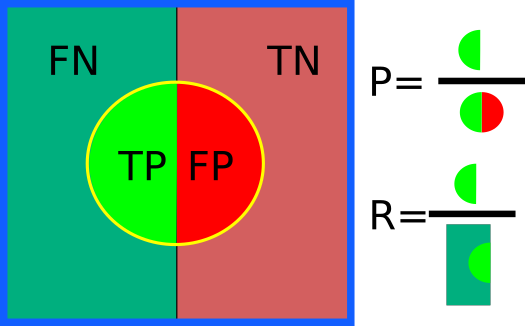
\includegraphics[width=0.6\linewidth] {evaluation/prec_recall}
\end{center}
\caption[Concept Recall and Precision]{This figure illustrates graphically the concept of Recall (\textbf{R}) and Precision (\textbf{P}). When estimating the sampling of a binary random variable, there are basically four possible outcomes: The we predicted it being true and it is true (\textbf{TP}), we predicted it true but it is false (\textbf{FP}), we predicted it false and it was actually negative (\textbf{FN}) or we predicted it to be true but it was actually false (\textbf{TN}). }
\label{fig:eval_concept_recall_precc}
\end{figure}
An alternative measure is the $F_1$ score. This measure is often used in determining the performance of classification tasks in machine learning. To compute its score, this measure takes into account both, the precision and the recall of the test. The exact definition of the F1 measure is given in equation $\ref{eq:f1_score}$.
\begin{equation}
F_1 = 2 \left( \frac{\text{precision} \times \text{recall}}{\text{precision} +\text{recall}} \right)
\label{eq:f1_score}
\end{equation}  
The F1 score can be interpreted as a normalized weighted average of the precision and recall measures. The best possible F1 score is equals 1 and its worst value is 0.

\section{Camera Model}
\subsection{Pinhole Camera}
A camera projects a 3d scene in a 2d image. A simple mathematical model to describe such a mapping from the 3d scene space to the 2d image space is the pinhole camera model. This model is conceptually illustrated in figure $\ref{fig:pinhole_camera_model}$.
\begin{figure}[H]
\begin{center}
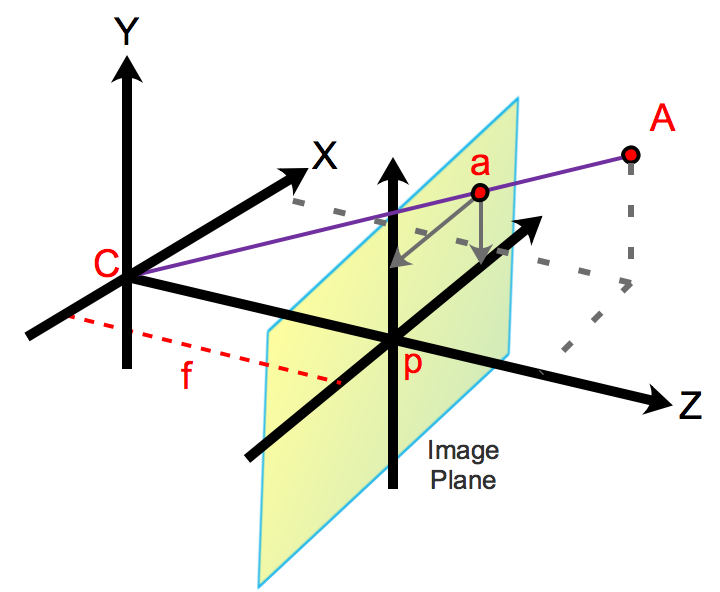
\includegraphics[width=0.8\linewidth] {background/camera_model/pinhole_camera}
\end{center}
\caption[Pinhole Camera Model]{Visualizing the pinhole camera model. The camera center $C$ represents an infinitely small aperture hole and assumed to be located at $(0,0,0)$, $f$ is the focal length in pixel units, $p$ is the principal point in images coordinates, $\textbf{A} = (X, Y, Z)$ a 3d point in the scene and $\textbf{a} = (f \frac{X}{Z}, f \frac{Y}{Z})$ its projected pixel version mapped onto the image plane.}
\label{fig:pinhole_camera_model}
\end{figure}
The aperture is an infinitely small hole and there is no lens used to focus light. Therefore, lens distorting or depth of field effects are ignored. The intersection point where all rays meet is the center of the perspective projection and usually referred by \textit{camera center}. The principal axis is formed by the line perpendicular to the image plane, which passes though the camera center. Its intersection point with the image plane is called principal point. The distance between the camera center and the principal point is the so called focal length.

\subsection{Camera Parameters}
\paragraph{Intrinsic Parameters} Let $\textbf{X} = (X,Y,Z,1)^T$ denote a point in a 3D scene and $\textbf{x} = (x,y,1)^T$ its projected version in the image plane. Both points are written in their homogeneous form. The mapping from a scene point to the image plane is defined as
\begin{equation}
\textbf{x} = 
\begin{pmatrix}
f & s & p_x & 0 \\
0 & f & p_y & 0 \\
0 & 0 & 1 & 0
\end{pmatrix}
\textbf{X}
\end{equation}
where $f$ denotes the focal length and $p = (p_x, p_y)^T$ the offset to the origin in image coordinates with respect to the principal point. In modern cameras, the skew $s$ is usually equals zero. The parameters $f$, $p_x$, $p_y$ and $s$ are called \textit{intrinsic camera parameters}. Notice, that $\textbf{X}$ is expressed in terms of camera coordinates and similarly, $\textbf{x}$ in pixel coordinates.

\paragraph{Extrinsic Parameters} In general, a camera is not located at the origin of the world coordinate system and can have an arbitrary orientation. Let $\textbf{X}_w$ denote a point, living in an arbitrary camera coordinate system. To express this point in the regular camera coordinate system, we have to apply a certain transformation. In a rigid object model, the points $\textbf{X}$ and $\textbf{X}_w$ can be transformed to one another by applying a linear transformation that consists of a rotational matrix $R$ and a translation $t$. The actual mapping is defined as
\begin{equation}
	X = \left[ R | t \right] X_w
\end{equation}
The parameters $t$ and $R$ are called \textit{extrinsic camera parameters}.

%%%
\chapter{Hole Filling}
\label{section:hole_filling}
In this section we address the problem of \emph{Hole Filling} by formulating this problem as a convex optimization. This formulation should enable us to generate dense segmentations from sparse segmentations. For solving the problem we develop and apply a primal-dual approximation. 
Given an image $g$ has missing information in form of holes, we want to find an optimal reconstructed image $u$. For describing the optimality property we take into account a cost function that describes the color smoothness and also that the resulting image $u$ should be close to the given raw input image $g$. \\ \\
More precisely, let $g$ denote a color image that exhibits holes. Then we want to solve for $u=(u_r, u_g, u_g)$ (RGB image) by minimzating the following energy term (cost function):
\begin{align}
	E(u_c) = \norm{\nabla u_c}_2 + \frac{\lambda}{2} \norm{u_c - g}^2_{\Omega_{c}}
\label{eq:basis_cost_demosaicing}	
\end{align}
with the measure
\begin{equation}
	\norm{u_C - g}^2_{\Omega_{C}} = \sum_x \sum_y \Omega_{C}(x,y)\norm{u_{c}(x,y) - g(x,y)}^2
\label{eq:measure}
\end{equation}
where C denotes the three different color channels. $\Omega_{C}$ is defined such that $\Omega_{C}(x,y) = 1$ if the pixel value at $(x,y)$ is \emph{valid}$\footnote{this means that the pixel at location (x,y) is valid for the bayer color mask C}$ and $\Omega_{C}(x,y) = 0$ when the data is missing. \\ \\
The cost function from equation $\ref{eq:basis_cost_demosaicing}$ consists of a smoothness term, $\norm{\nabla u_c}_2$ and $\norm{u_c - g}^{2}_{\Omega_{c}}$. The first term ensures a smooth color transition between colors in a l2 norm sense. The second term ensures that the reconstructed images does not deviate too much from the given input, i.e. de demosaiced image should resemble to the provided mosaiced raw camera image. This similarity term is further parameterized by a regularization term $\lambda$, indicating how strong the output should match the given input according to the formulated measure in equation $\ref{eq:measure}$. In summary, larger values for $\lambda$ weight the similarity of the input and output image more, and contrarely, lower values weight the color smoothness term more. \\ \\
Hereby, minimizating the cost function from equation $\ref{eq:basis_cost_demosaicing}$ leads to an optimal demosaiced image $u$.
Mathematically we want to solve for 

\begin{equation}
	\widetilde{u} = \argmin_{u_c} E(u_c)
\label{eq:our_general_cost_function}
\end{equation}
We can further simplify the cost function stated in equation $\ref{eq:basis_cost_demosaicing}$ relying on the following observation: Since the function $\Omega_{C}$ is only true for pixels that correspond to the color channel C in the bayer mask, we see that 
\begin{equation}
	\Omega_{C}(x,y)\norm{u_{c}(x,y) - g(x,y)}
\end{equation}
is only not equal zero if the pixel at location $(x,y)$ belongs to the color channel $C$. Therefore we are allowed to solve the stated optimization problem from equation $\ref{eq:basis_cost_demosaicing}$ for each color channel separately. 


According to this insight we are supposed to minimize the following three independent$\footnote{Independent in the sense that we are allowed to solve for each color channel separately}$ convex problems:



\begin{align}
	\widetilde{u}_R = \argmin_{u_R} \norm{\nabla u_R}_2 + \frac{\lambda}{2} \norm{u_R - g}^2_{\Omega_{R}} \nonumber \\
	\widetilde{u}_G = \argmin_{u_G} \norm{\nabla u_G}_2 + \frac{\lambda}{2} \norm{u_G - g}^2_{\Omega_{G}}\nonumber \\
	\widetilde{u}_B = \argmin_{u_B} \norm{\nabla u_R}_2 + \frac{\lambda}{2} \norm{u_B - g}^2_{\Omega_{B}}
\label{eq:our_convex_probelm}		
\end{align}

Where we still rely on the measure defined in equation $\ref{eq:measure}$ but C was replayed by the appropriate color channel$\footnote{C stands for either the color channel R, G or B.}$. We notice that the equations in $\ref{eq:our_convex_probelm}$ tell us that we have to solve three different energies similar to the one formulated in equation $\ref{eq:our_general_cost_function}$.

In the next section we will describe how to solve the stated minimization problems from equation $\ref{eq:our_convex_probelm}$ numerically.

\section{Primal-Dual Form}
In this section we derive the primal-dual form of the stated convex demosaicing problem.

But first off, let us consider an initial problem of the form 

\begin{align}
	\min_{x \in X} F(K x) + G(x)
\label{eq:initial_primal}	
\end{align}

where $F$, $G$ are convex functions and $K$ denotes a linear operator. 

The primal-dual formulation for equation $\ref{eq:initial_primal}$ is given by 

\begin{align}
	\min_{x \in X} \max_{y \in Y} < Kx, y > - F^*(y) + G(x)
\label{eq:initial_primal_dual}	
\end{align}


For a given mosaiced RGB image $u_{RGB}$ encoded as a 3 dimensional $M \times N$ matrix, i.e. a tensor of dimension $M \times N \times 3$. As mentioned in the problem statement we can solve three independent convex problems in order to solve the problem of demosaicing a RGB image. Therefore let in the following $u$ define stand for one particular color channel of the given color image $u_{RGB}$.

\begin{equation}
\min_{u \in U} \norm{\nabla u} + \frac{\lambda}{2} \norm{u - g}^2_{\Omega}
\label{eq:initial_energy}
\end{equation}

where $\norm{u - g}^2_{\Omega}$ is defined as in equation $\ref{eq:measure}$ and $g$ is the corresponding color channel of the mosaiced image described in the problem statement.

We observe that equation $\ref{eq:initial_energy}$ has the same structure as the initial problem stated in equation $\ref{eq:initial_primal}$. This allows us to formulate the primal-dual form of equation $\ref{eq:initial_energy}$ which will look like the following:

\begin{align}
	\min_{u \in U} \max_{y \in Y} < Kx, y > - F^*(y) + G(x)
\label{eq:initial_primal_dual}	
\end{align}

Where $K$, $F$ and $G$ are defined as:

\begin{align}
	K &= \nabla \nonumber \\
	F &= \norm{\cdot}_2 \nonumber \\
	G &= \norm{u - g}^2_{\Omega}
\label{eq:def_kfg}	
\end{align}

Note that $F*$ denotes the convex conjugate form of $F$. The convex conjugate of $F$ has an explicit identity that can be computed using the Legendre-Fenchel-Transform.

\begin{align}
	F^*(y) &= (\norm{\cdot}_2)^*(y) \nonumber \\
		  &= \sup_x x^T y - \twonorm{x} \nonumber \\
		  &= \sup_x x^T y - \max_{\twonorm{z} \leq 1} x^T z \nonumber \\
		  &= \sup_x \min_{\twonorm{z} \leq 1} x^T(y-z) \nonumber \\
		  &= \begin{cases}
   				0  			& \text{if} \twonorm{y} \leq 1 \\
   				\infty      & \text{otherwise}
  			 \end{cases} \nonumber \\
  		  &= \delta(y)
\label{eq:legendre_fenchel_transform_f}  		  
\end{align}

The first equality is simply the definition of $F$. The second equality is using the so called Legendre-Fenchel transformation,

\begin{equation}
	(\norm{\cdot}_2)^*(y) = \sup_x x^T y - \twonorm{x} \nonumber
\end{equation}. 

In the third equality I make use of the Cauchy-Schwarz inequality, 
\begin{equation}
	\twonorm{x} = \max_{\twonorm{z} \leq 1} x^T z
\end{equation}


Plugging equation $\ref{eq:legendre_fenchel_transform_f}$ and the definitions in from equation $\ref{eq:def_kfg}$ into the primal-dual equation equation $\ref{eq:initial_primal_dual}$ we conclude the following final primal-dual formulation:

\begin{equation}
\min_{u \in U} \max_{y \in Y} <\nabla u, y> - \delta(y) + \frac{\lambda}{2}\norm{u - g}^2_{\Omega}
\label{eq:final_primal_dual}
\end{equation}


\section{Primal-Dual steps}
In this section I will present an iterative solver for our stated primal-dual formulation.

In the following I am going to rely on an algorithm $\cite{chambolle2011first}$ formulated by A.Chambolle and T.Pocke, which allows to solve primal-formulations as ours stated in equation $\ref{eq:final_primal_dual}$.
They stated an iterative algorithm that has the following update steps:

\begin{align}
	y^{n+1} &= \prox_{\sigma F^*}(y^n + \sigma K \bar{x}^n) \nonumber \\
	x^{n+1} &= \prox_{\tau G}(x^n - \tau K^* y^{n+1}) \\
	\bar{x}^{n+1} &= x^{n+1} + \theta(x^{n+1} - x^n)
\label{eq:update_rules_plain}	
\end{align}
with $\theta \in (0, 1]$ and the constraint $\tau \sigma \norm{K}^2 < 1$. Note that stated constraint is important in order to guarantee convergence of their algorithm.

Hereby $prox(\cdot)$ denotes the proximity operator and is defined as 

\begin{equation}
	\prox_{\lambda F}(z) = \arg \min_x \frac{1}{2} \twonorm{x - z}^2 + \lambda F(x)
\end{equation}

In the following we will derive explicit identities for the update rules in equation $\ref{eq:update_rules_plain}$that can be numerically solved. Our goal is to find an expression for the proximity operator.

\section{Update for $y^{n+1}$}

In this subsection we derive an identity for the $y^{n+1}$ update rule from equation $\ref{eq:update_rules_plain}$. The key idea is to use the so called Moreau's Identity:  

\begin{equation}
	\prox_{\lambda F^*}(z) = z - \lambda \cdot \prox_{F/ \lambda}(z / \lambda) 
\label{eq:moreau}	
\end{equation}

Next, we apply the Moreau's identity to the proximity operator of the Legendre-Fenchel transformation.


\begin{align}
	\prox_{\lambda F^*}(y^n + \sigma K \bar{x}^{n}) 
	&= (y^n + \sigma K \bar{x}^{n}) - \sigma \prox_{\frac{F}{\sigma} } \left(\frac{y^n + \sigma K \bar{x}^{n} }{\sigma} \right) \nonumber \\
	&= (y^n + \sigma K \bar{x}^{n}) - \sigma \left( \frac{y^n + \sigma K \bar{x}^{n} }{\sigma} \max{0, 1-\frac{1}{\twonorm{y^n + \sigma K \bar{x}^{n} }}} \right) \nonumber \\
	&= (y^n + \sigma K \bar{x}^{n}) - \left( y^n + \sigma K \bar{x}^{n} \right) \max{\left(0, 1-\frac{1}{\twonorm{y^n + \sigma K \bar{x}^{n} }}\right)}  
\label{eq:y_n_1_expression}
\end{align}

For the first equality we use the definition of equation $\ref{eq:moreau}$ and for the second equality we used the fact (proven during class) that

\begin{align}
	\prox_{\frac{\twonorm{\cdot}}{\sigma}}(\frac{x}{\sigma}) = \frac{x}{\sigma} \max{\left(0, 1-\frac{1}{\twonorm{x}}\right)}
\end{align}

To simplify our derivation even and also get rid of the proximity operator we next make a case distinction for $\twonorm{y^n + \sigma K \bar{x}^{n}}$. 

\begin{itemize}
	\item If $\twonorm{y^n + \sigma K \bar{x}^{n}} \geq 1$
		then  
		\begin{align}
			0 \leq 1-\frac{1}{\twonorm{y^n + \sigma K \bar{x}^{n}}} \leq 1
		\end{align}
		
		Therefore $\frac{1}{\twonorm{y^n + \sigma K \bar{x}^{n}}}$ is smaller than one and thus
		
		\begin{align}
			\max{\left(0, 1-\frac{1}{\twonorm{y^n + \sigma K \bar{x}^{n}}}\right)} 
			&= 1-\frac{1}{\twonorm{y^n + \sigma K \bar{x}^{n}}}
		\end{align}
		
		This insight can directly be used for the maximum expression in equation $\ref{eq:y_n_1_expression}$ and we hence obtain:
		
		\begin{align}
			\prox_{\lambda F^*}(y^n + \sigma K \bar{x}^{n})
			&= (y^n + \sigma K \bar{x}^{n}) - \left( y^n + \sigma K \bar{x}^{n} \right) \max{\left(0, 1-\frac{1}{\twonorm{y^n + \sigma K \bar{x}^{n} }}\right)} \nonumber \\
			&= (y^n + \sigma K \bar{x}^{n}) - \left( y^n + \sigma K \bar{x}^{n} \right) \left( 1-\frac{1}{\twonorm{y^n + \sigma K \bar{x}^{n}}} \right)\nonumber \\
			&= (y^n + \sigma K \bar{x}^{n}) -(y^n + \sigma K \bar{x}^{n}) +\frac{y^n + \sigma K \bar{x}^{n}}{\twonorm{y^n + \sigma K \bar{x}^{n}}} \nonumber \\
			&= \frac{y^n + \sigma K \bar{x}^{n}}{\twonorm{y^n + \sigma K \bar{x}^{n}}}
		\end{align}
		
	\item If $\twonorm{y^n + \sigma K \bar{x}^{n}} < 1$
		then 
		\begin{align}
			1-\frac{1}{\twonorm{y^n + \sigma K \bar{x}^{n}}} < 0
		\end{align}
		thus we conclude 
		\begin{align}
			\max{\left(0, 1-\frac{1}{\twonorm{y^n + \sigma K \bar{x}^{n}}}\right)} 
			&= 0
		\end{align}
		which offers us the following new identity for equation $\ref{eq:y_n_1_expression}$:
		
		\begin{align}
			\prox_{\lambda F^*}(y^n + \sigma K \bar{x}^{n})
			&= (y^n + \sigma K \bar{x}^{n}) - \left( y^n + \sigma K \bar{x}^{n} \right) \max{\left(0, 1-\frac{1}{\twonorm{y^n + \sigma K \bar{x}^{n} }}\right)} \nonumber \\
			&= (y^n + \sigma K \bar{x}^{n}) - \left( y^n + \sigma K \bar{x}^{n} \right) 0 \nonumber \\
			&= y^n + \sigma K \bar{x}^{n}
		\end{align}
\end{itemize}

By using the results from the case distinction from above we can simplify equation $\ref{eq:y_n_1_expression}$ even further to:

\begin{equation}
	\prox_{\lambda F^*}(y^n + \sigma K \bar{x}^{n}) = \frac{y^n + \sigma K \bar{x}^{n}}{\max{\left(1,\twonorm{y^n + \sigma K \bar{x}^{n}} \right)}}
\label{eq:y_p_1_we_proxy}	
\end{equation}

Finally, the only left step to do is to plug in the definition of $K$ into equation $\ref{eq:y_p_1_we_proxy}$ which gives us then the final update rule for $y_{n+1}$ when relying on the update rule from equation $\ref{eq:y_n_1_expression}$:

\begin{align}
	y_{n+1} = \frac{y^n + \sigma \nabla \bar{x}^{n}}{\max{\left(1,\twonorm{y^n + \sigma \nabla \bar{x}^{n}} \right)}}
\label{eq:update_rule_y_n_p_1}	
\end{align} 	

\section{Update for $x^{n+1}$}

\begin{align}
x^{n+1} &= \prox_{\tau G}(x^n - \tau K^* y^{n+1}) \\
		&= \prox_{\tau \frac{\lambda}{2} \norm{u - g}_{\Omega}^2 }(x^n - \tau \nabla^* y^{n+1}) \\
	    &= \arg \min_{z} \frac{1}{2} \twonorm{\left(x^n - \tau \nabla^* y^{n+1} \right) - z}^2 + \tau \frac{\lambda}{2}\norm{z - g}_{\Omega}^2 \\
	    &= \arg \min_{z} E(z)
\label{eq:energy_x_p_1}	    
\end{align}

To simplify the following derivations, let us define the following substitution: 
\begin{align}
	m := \left(x^n - \tau \nabla^* y^{n+1} \right)
\end{align}

We can solve for $x^{n+1}$ by finding the zeros of the partial derivative of $E(z)$ from equation $\ref{eq:energy_x_p_1}$. Let us start with the partial derivative along $z$ of $E(z)$ from equation $\ref{eq:energy_x_p_1}$: 

\begin{align}
	\partial_{z} E(z)
	&= \partial_{z} \left( \frac{1}{2} \twonorm{m - z}^2 + \tau \frac{\lambda}{2}\norm{z - g}_{\Omega}^2 \right) \nonumber \\
	&= \frac{1}{2} \partial_{z} \left[ \left( m - z \right)^{T}\left( m - z \right) + \tau \lambda \Omega \left( z -g \right)^{T}\left( z -g \right) \right] \nonumber \\
	&= \frac{1}{2} \partial_{z} \left[ m^{T}m -2m^{T} z + z^{T} z + \tau \lambda \Omega \left( z^{T}z -2z^{T} g + g^{T} g\right) \right] \nonumber \\
	&= \frac{1}{2} \left[ -2m + 2z + \tau \lambda \Omega \left( 2 z -2g \right) \right] \nonumber \\
	&= \left[ -m + z + \tau \lambda \Omega z - \tau \lambda \Omega g \right]	 \nonumber \\	
	&= \left[ \left(1+\tau \lambda \Omega \right)z-m - \tau \lambda \Omega g \right]	 \nonumber \\
\label{eq:derivative_x_n_p_1}		
\end{align}

Next, let us set the finding from equation $\ref{eq:derivative_x_n_p_1}$ to zero and solve for $z$:

\begin{align}
	\partial_{z} E(z) 
	&= 0 \nonumber \\
	&\Leftrightarrow \left(1+\tau \lambda \Omega \right)z-m - \tau \lambda \Omega g = 0 \nonumber \\
	&\Rightarrow z = \left(m +  \tau \lambda \Omega g \right) \left( 1+\tau \lambda \Omega\right)^{-1} \nonumber \\
	&\Rightarrow z = \frac{m +  \tau \lambda \Omega g}{1+\tau \lambda \Omega} \nonumber \\
\label{eq:zeros_ez}	
\end{align}

Note that the division $(1+\tau \lambda \Omega)$ denotes a component-wise division, since $\Omega$ is applied component-wise to the elements of $g$. In addition, 1 and $\Omega$ are representing matrices here (of same dimension as $g$ and $z$ ($u$ respectively).

By plugging the definition $m$ into equation $\ref{eq:zeros_ez}$ and using the fact, that $z$ corresponds to $x^{n+1}$ we can conclude:

\begin{align}
	x^{n+1} 
	&= \frac{x^n - \tau \nabla^* y^{n+1} +  \tau \lambda \Omega g}{1+\tau \lambda \Omega} \nonumber \\
	&= \frac{x^n + \tau div(y^{n+1}) +  \tau \lambda \Omega g}{1+\tau \lambda \Omega}
\label{eq:update_x_n_p_1}	
\end{align}

In the last step we used the well known fact, that 
\begin{align}
	\nabla^* (v) = -div(v)
\end{align}

for any vector-field $v$ of the form 

\begin{align}
	v = \nabla u
\end{align}


